\subsubsection{Descripción y grafo de relación entre los nodos}

Realizamos una captura en la red Wi-Fi \emph{Entrepiso-DC}, disponible desde los laboratorios del Depto. de Computación. La muestra fue tomada un lunes a las 17hs aproximadamente -horario típicamente de alto tráfico-, logrando un total de XX paquetes en MM minutos.

En el gráfico de la figura \ref{fig:entrepiso-dc-grafo} se presenta el grafo dirigido representando la red. En el mismo se observa una gran cantidad de nodos ligada al nodo con IP 10.1.200.197, y luego múltiples conjuntos pequeños de nodos conectados entre sí pero disconexos de la estructura mayoritaria.

\begin{figure}[H]
  \begin{center}
    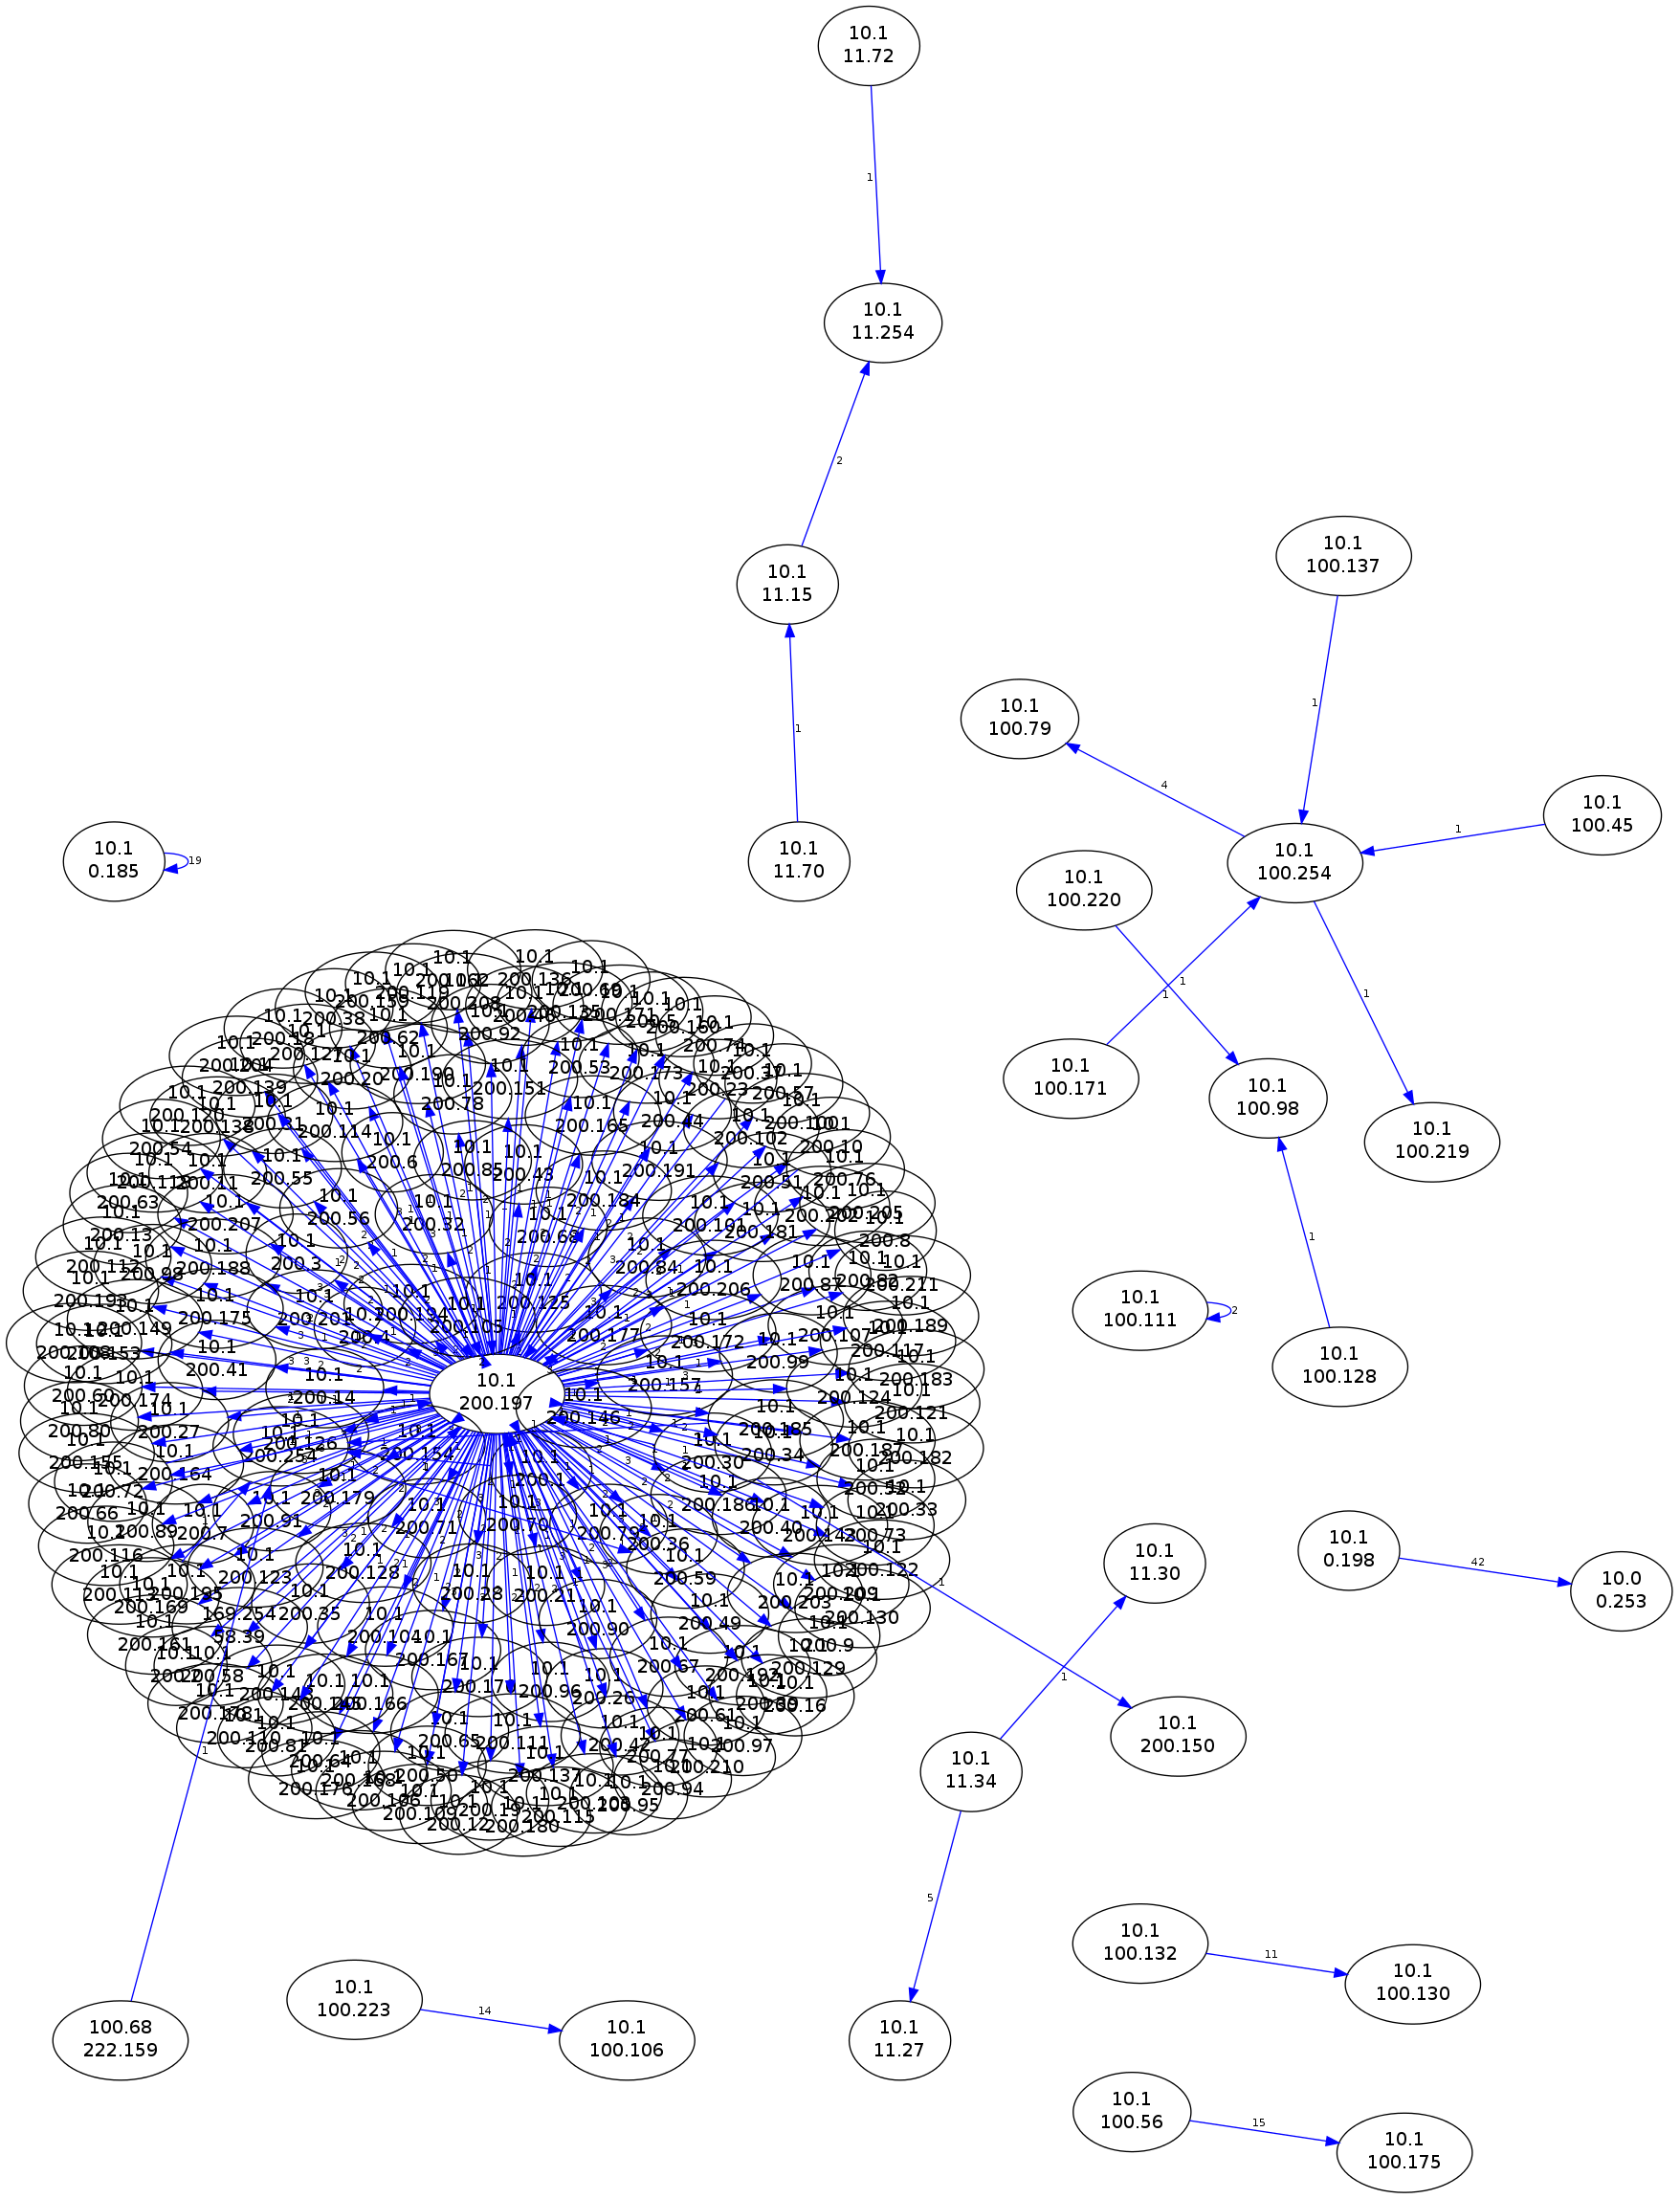
\includegraphics[width=0.6\linewidth]{../imgs/red-entrepiso-dc_red.png}
    \caption{Grafo mostrando la topología de la red \emph{Entrepiso-DC}.}
    \label{fig:entrepiso-dc-grafo}
  \end{center}
\end{figure}

\subsubsection{Fuente: $S_{dst}$}

\begin{figure}[H]\centering
    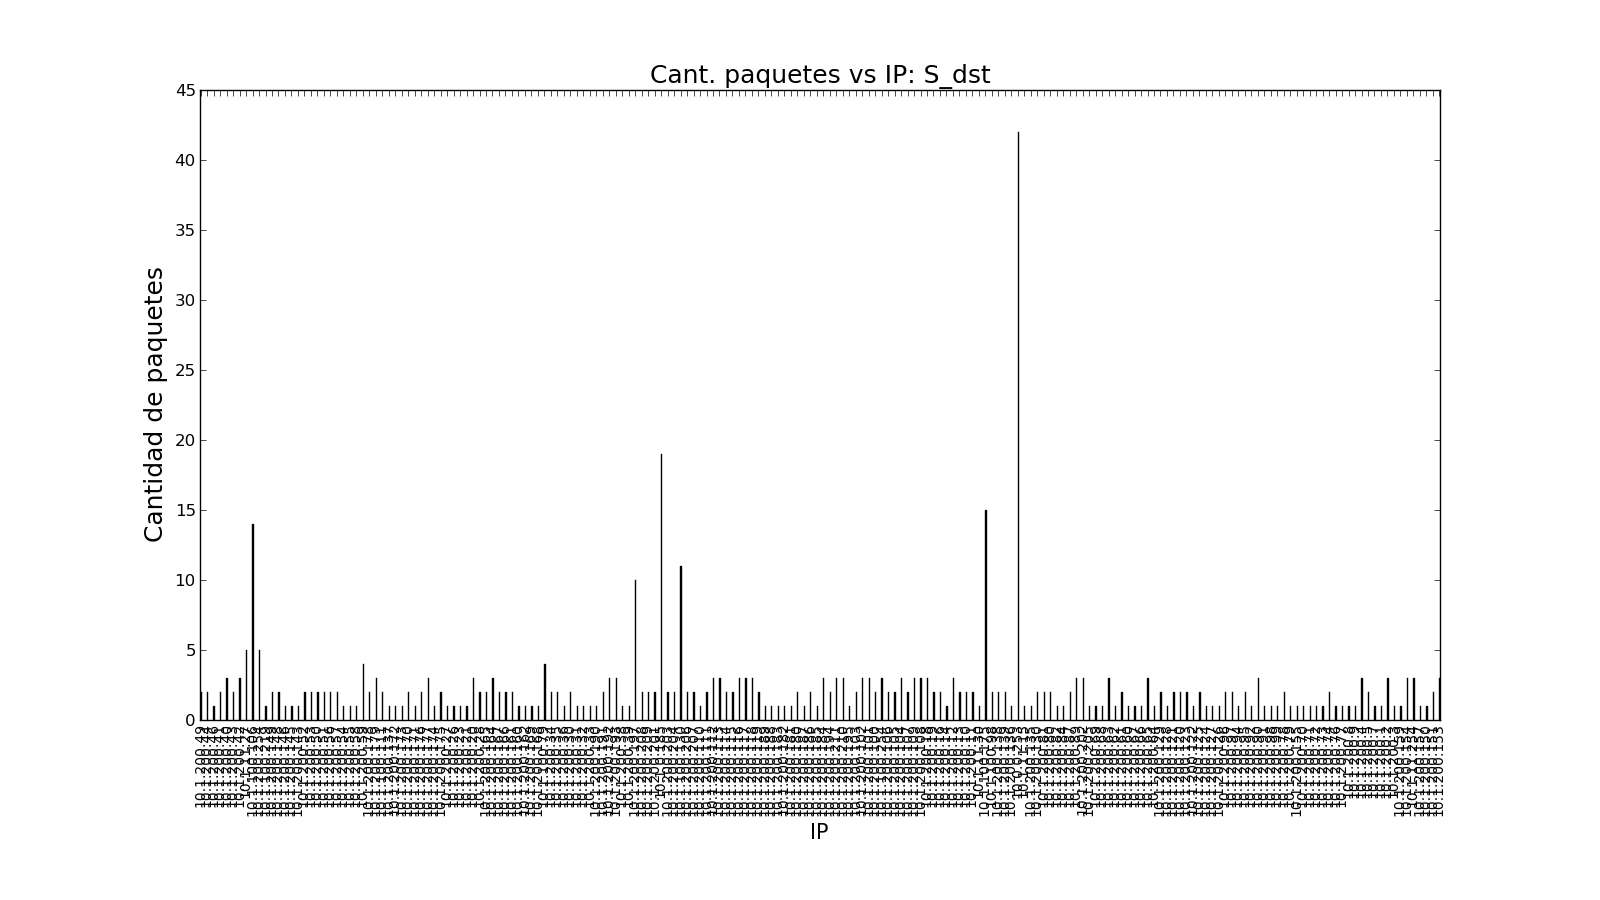
\includegraphics[width=\linewidth]{../imgs/red-entrepiso-dc_S_dst_hist.png}
    \caption{Histograma de $S_{dst}$}\label{fig:entrepiso-dc-dst-hist}
\end{figure}

\begin{figure}[H]\centering
    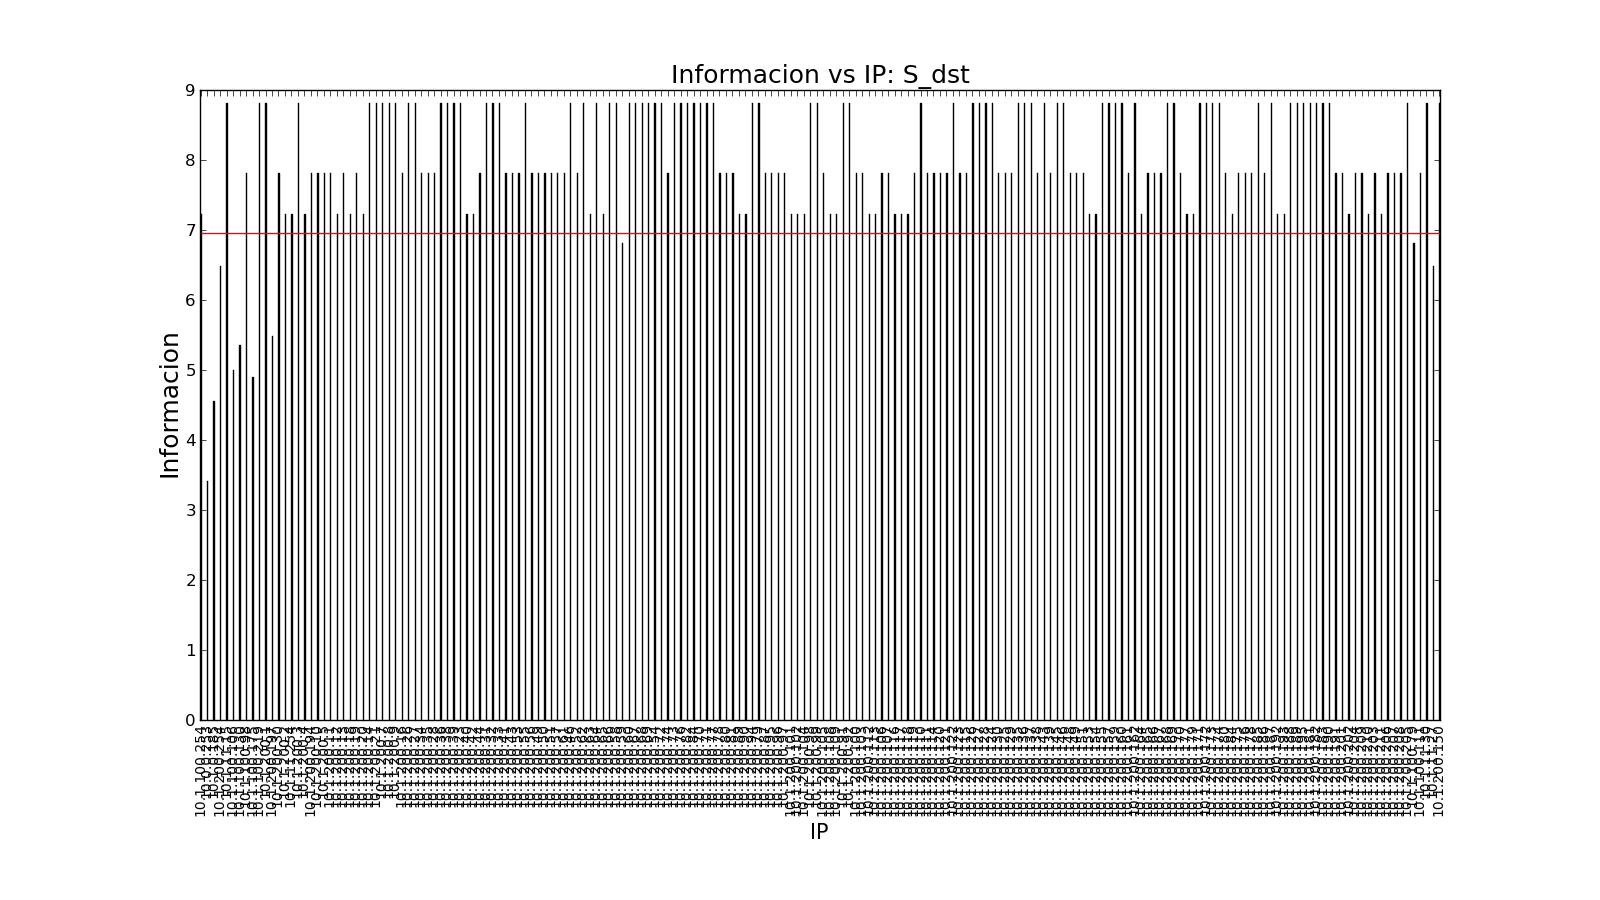
\includegraphics[width=\linewidth]{../imgs/red-entrepiso-dc_S_dst_info.png}
    \caption{Informacion de $S_{dst}$}\label{fig:entrepiso-dc-dst-info}
\end{figure}

$\bullet$ Entropía de la fuente: 6.95922916897

\subsubsection{Fuente: $S_{src}$}

\begin{figure}[H]\centering
    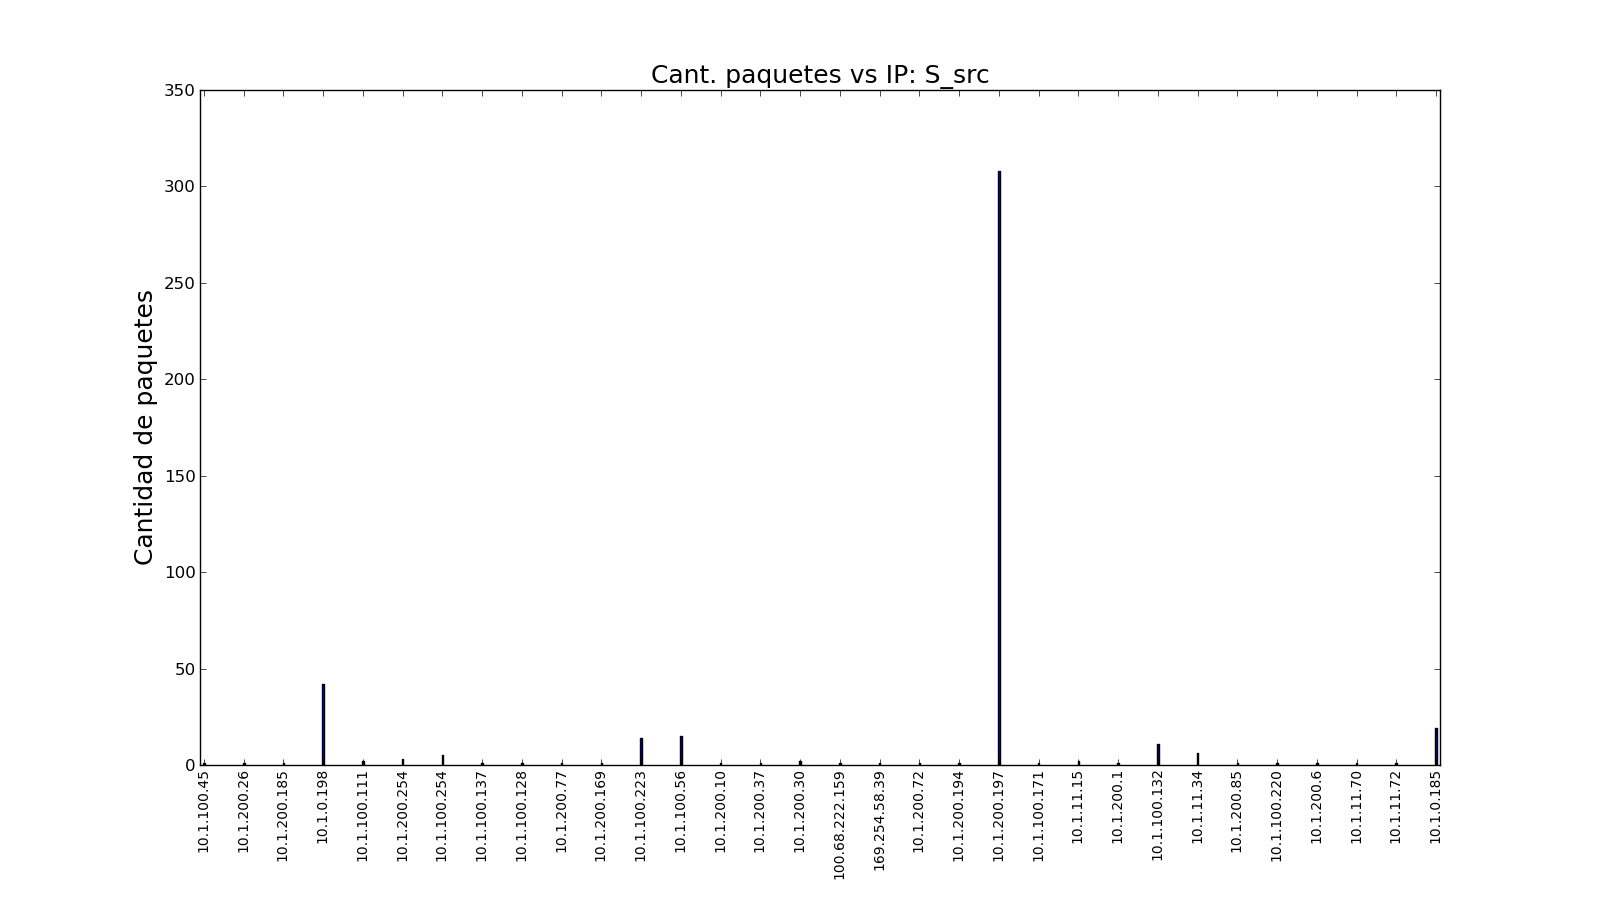
\includegraphics[width=\linewidth]{../imgs/red-entrepiso-dc_S_src_hist.png}
    \caption{Histograma de $S_{src}$}\label{fig:entrepiso-dc-src-hist}
\end{figure}

\begin{figure}[H]\centering
    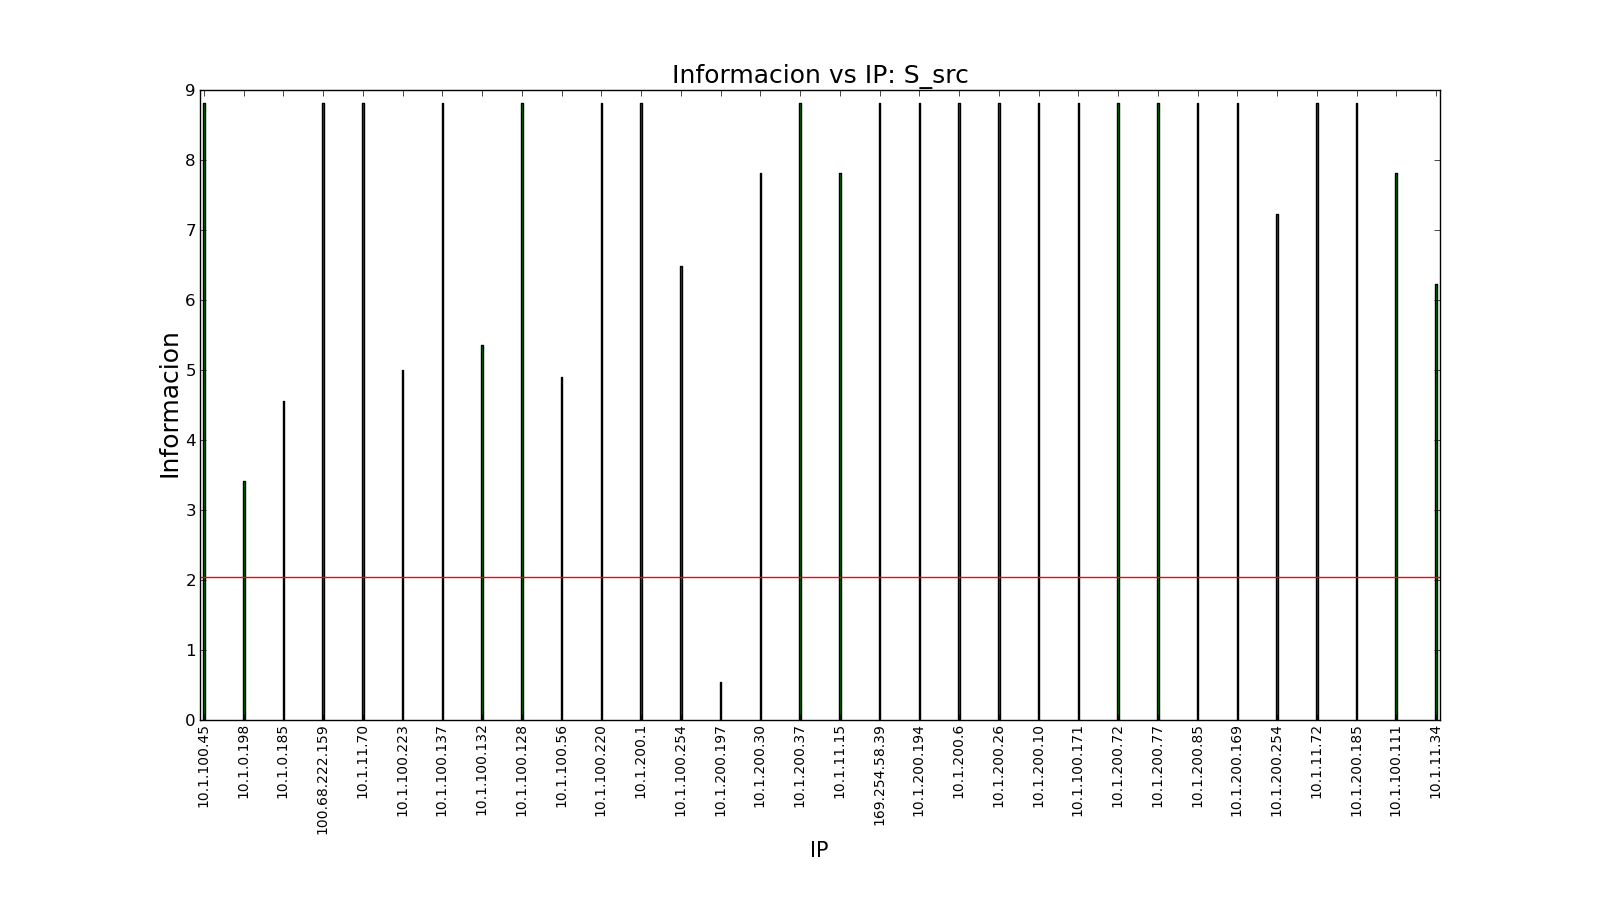
\includegraphics[width=\linewidth]{../imgs/red-entrepiso-dc_S_src_info.png}
    \caption{Informacion de $S_{src}$}\label{fig:entrepiso-dc-src-info}
\end{figure}

$\bullet$ Entropía de la fuente: 2.03731420117

\subsubsection{Discusión}

cualquier cosa interesante sobre este caso en particular